\section{Reducing the Stepsize}
\label{sec:reducing_stepsize}

For the results shown in this section a stepsize of $0.2$s has been used for the MPC. This stepsize returns smooth stable paths for most of the curved paths, but do not work well with the sharper corners in the linear paths. Testing showed that by decreasing the timestep to $0.1$s, the MPC manages to return a stable flight path for linear corners with a $70\degree$ angle. The MPC was still not able to return a stable flight path for $90\degree$ linear turns.

Figure \ref{fig:70deg_lin_error} shows the result of optimizing a linear $70\degree$ turn with a stepsize of $0.1$s. Even though the MPC returns a stable flight path, it can be seen that the camera contains many small oscillations. By closer inspection of Figure \ref{fig:70deg_lin_roll_error}, it can be seen that the roll angle of the aircraft oscillates throughout the entire flight.

\begin{figure}
	\makebox[\textwidth][c]{
	\subfloat[UAV position][UAV position.]{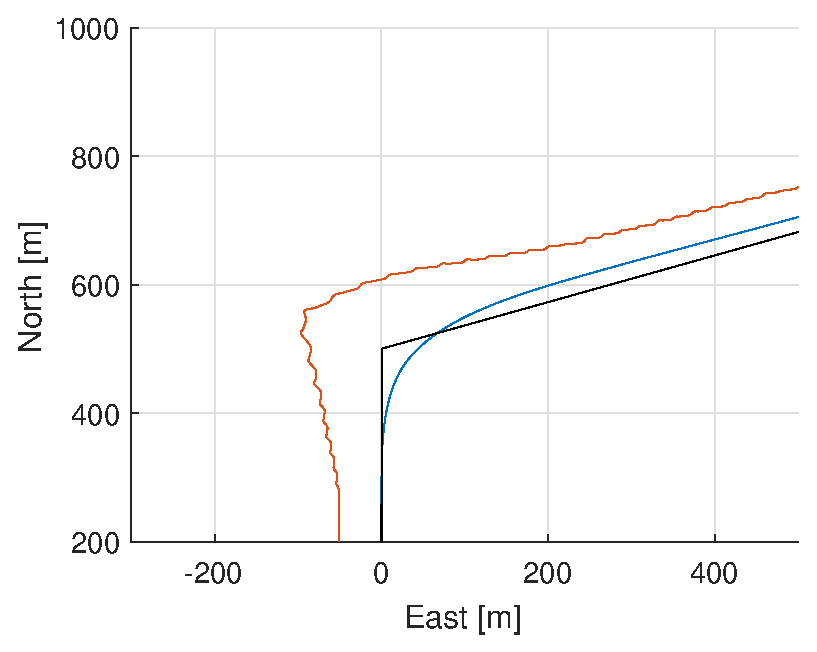
\includegraphics[width=0.5\textwidth, keepaspectratio=true]{../../results/opt/error/fig_70deg/uav_pos_1.eps}}
	\qquad
	\subfloat[Camera position][Camera poistion.]{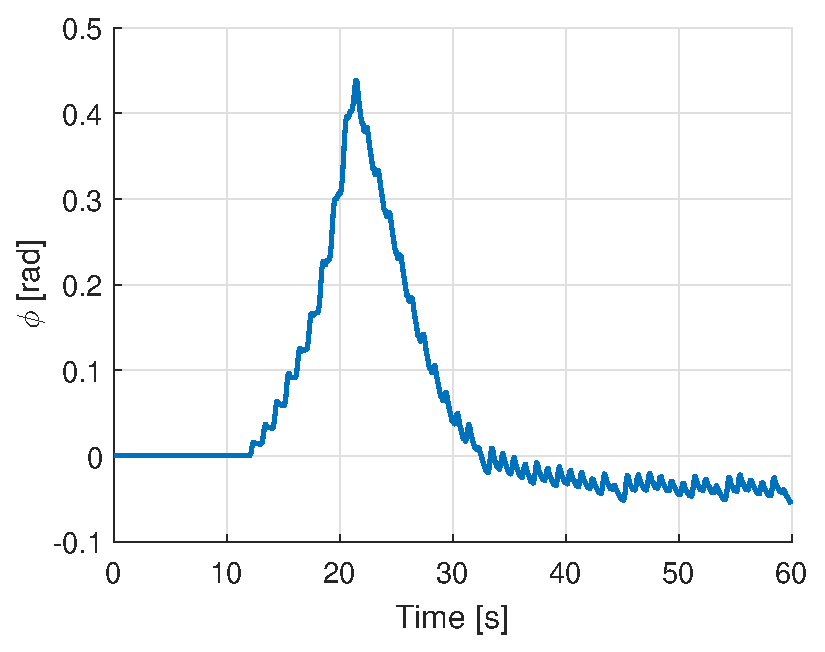
\includegraphics[width=0.5\textwidth, keepaspectratio=true]{../../results/opt/error/fig_70deg/uav_phi_1.eps}
    \label{fig:70deg_lin_roll_error}}}
	\caption{Results of optimizing a curved $70\degree$ turn.}
	\label{fig:70deg_lin_error}
\end{figure}